
In any 3D application, mathematical models are used to represent the positions, rotations and scale of objects within a given scene. It is important for the purpose of this thesis to briefly touch on some of the core concepts, particularly with regards to representing the position and rotation of 3D objects. All objects within a 3D application are represented by a set of vertices or points, which can be represented with X, Y and Z coordinates. Three vertices can make up one triangle also called a face, multiple faces will then make up a whole 3D object. The use of mathematical methods in 3D graphics is to be able to manipulate all vertices of an object in a consistant way, thus rotating, translating or scaling the object within the scene. This section will provide sufficient background on some of most important concepts of 3D Mathematics, such as vectors, matrices and quaternions, which are widely used in the turtle graphics interpreter as well as the model generator.

\section{Vectors}

Vectors have many meanings in different contexts, in \acrshort{3d} computer graphics, often vectors are refering to the Euclidean vector. The Euclidean vector is a quantity in $n$-dimensional space that has both magnitude (the length from A to B) and direction (the direction to get from A to B). Vectors can be represented as a line segment pointing in a direction, with a certain length. A \acrshort{3d} vector can be written as a triple of scalar values eg: $(x, y, z)$

The most common operations on vectors are multiplication by a scalar, addition, subtraction, normalisation and the dot and cross product. The multiplication by a scalar value can be simply seen as scaling the magnitude of the vector itself, this can be done uniformly or non-uniformly as seen in the equation below:

\begin{equation}
a \otimes s = (a_x s_x, a_y s_y, a_z s_z)
\end{equation}

\noindent
Where $\otimes$ is the component-wise product of a vector $a$ and the scaling vector $s$. Similar to the scalar product of a vector the addition and subtraction of two vectors is the component-wise sum or difference. 

\begin{equation}
\begin{aligned}
a \oplus b = [(a_x + b_x), (a_y + b_y), (a_z + b_z)]\\
a \ominus b = [(a_x - b_x), (a_y - b_y), (a_z - b_z)]
\end{aligned}
\end{equation}

\begin{figure}[htbp]
	{\centering
		\setlength{\fboxrule}{1pt}
		\vspace{7px}
		\fbox{
			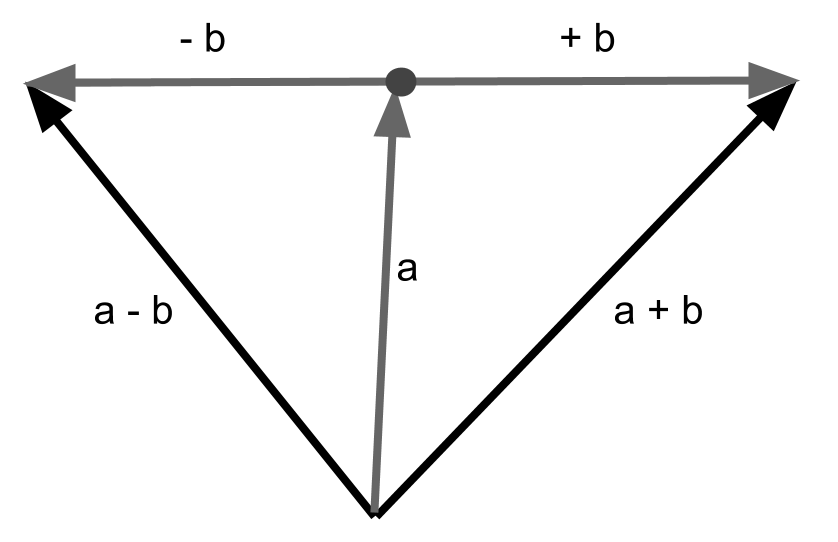
\includegraphics[scale=0.2]{Diagrams/vector_addition.png}
			\label{3DAxisFigure}
		}
		\caption{Table of common dot product tests between two vectors.}
	}
\end{figure}
\FloatBarrier

\noindent
A useful type of vector is known as a unit vector. This is a type of vector which has a magnitude of 1. Unit vectors are used extensively in computer graphics particularly with ragards to \gls{Shader}s. Take the vector v its magnitude $\alpha$ can be calculated by taking the square root of the product its components squared, as seen below 

\begin{equation}
	\alpha =~ \mid \textbf{v} \mid~ = \sqrt{\textbf{v}^2_x + \textbf{v}^2_y + \textbf{v}^2_z}
\end{equation}

The unit vector can then be calculated by taking the product of $v$ and the reciprocal of its magnitude shown in the following equation.

\begin{equation}
	\upsilon = \frac{\textbf{v}}{\alpha} = \frac{1}{\alpha} \textbf{v}
\end{equation}

There are many different ways to multiply vectors, however, in 3D graphics there two main multiplications. These being the dot and cross product. The dot product yields a scalar by adding the products of the vector product components. The cross product on the other hand is the product of two vectors which gives a vector which is perpendicular. The dot product can be calculated using the formula below: 

\begin{equation}
a \cdot b = a_x b_x + a_y b_y + a_z b_z = d
\end{equation}

\noindent
Some of the main uses for dot products within 3D graphics is to find whether two vectors are collinear, perpendicular, in the same direction or opposite directions. One possible use for this is to find the dot product of two branches directions in order to find out if they growing in the same direct or in opposite directions. In the table \ref{dot product test} below, there are each of the dot product test diagrams as well as the test equation where $ab = \mid a \mid \mid b \mid = a \cdot b$.

\begin{table}[h!]
\centering
\begin{tabular}{ | c | c | c |}
\hline
	Test 	& Equation & Example\\  
\hline
\hline
	Collinear 							& $(a \cdot b) = ab$ & 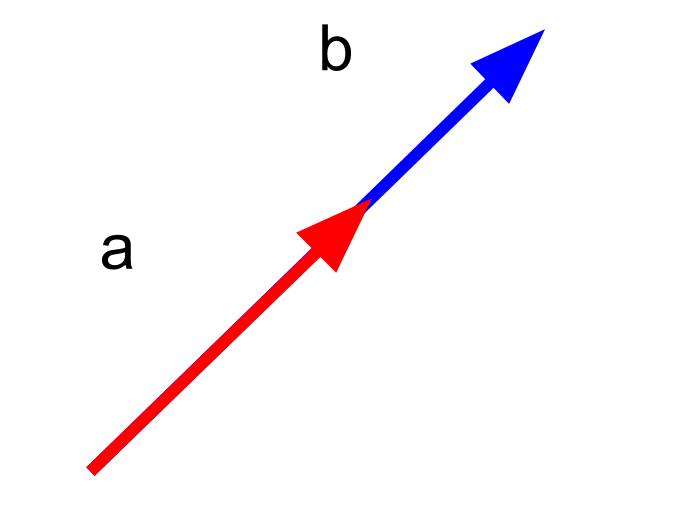
\includegraphics[scale=0.1]{Diagrams/vector1.png}\\
\hline
	Opposite Collinear 					& $(a \cdot b) = -ab$ &	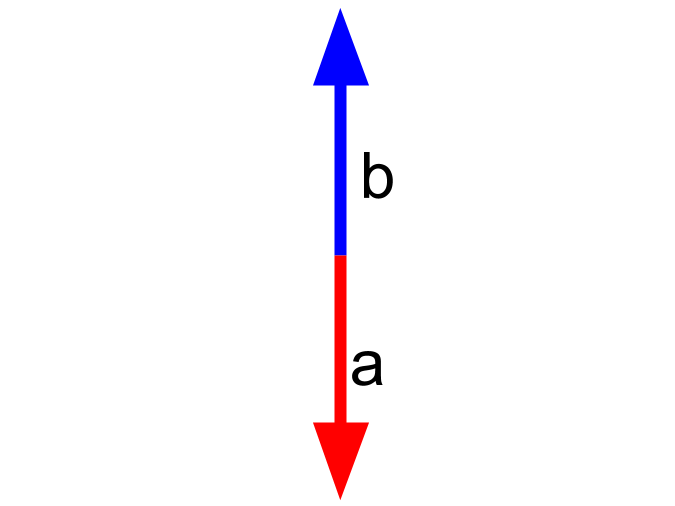
\includegraphics[scale=0.1]{Diagrams/vector2.png}\\
\hline
	Perpendicular 						& $(a \cdot b) = 0$	&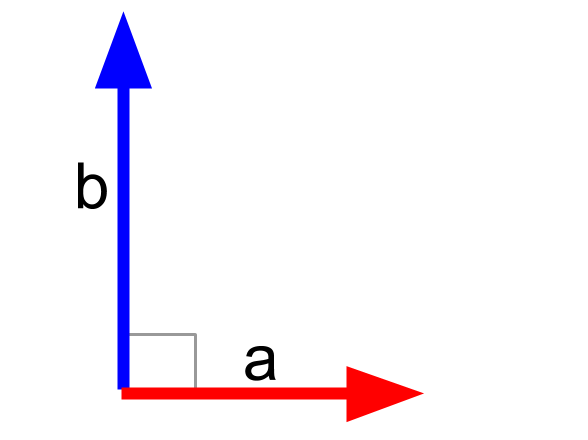
\includegraphics[scale=0.1]{Diagrams/vector3.png}\\
\hline
	Same Direction 						& $(a \cdot b) > 0$ &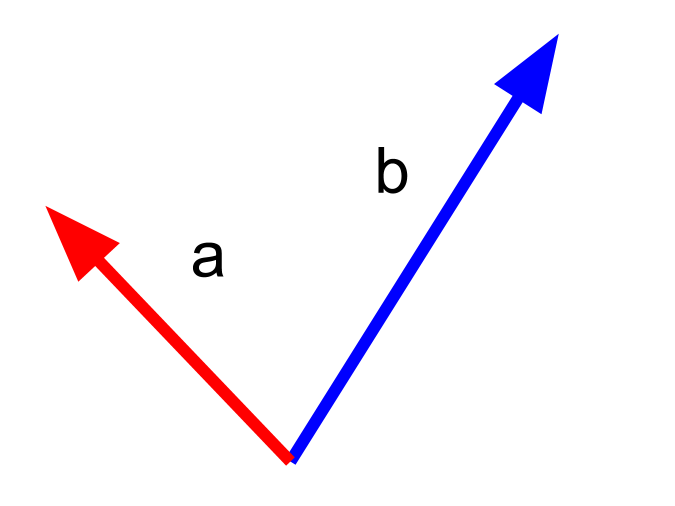
\includegraphics[scale=0.1]{Diagrams/vector4.png}\\
\hline
	Opposite Direction 					& $(a \cdot b) < 0$ &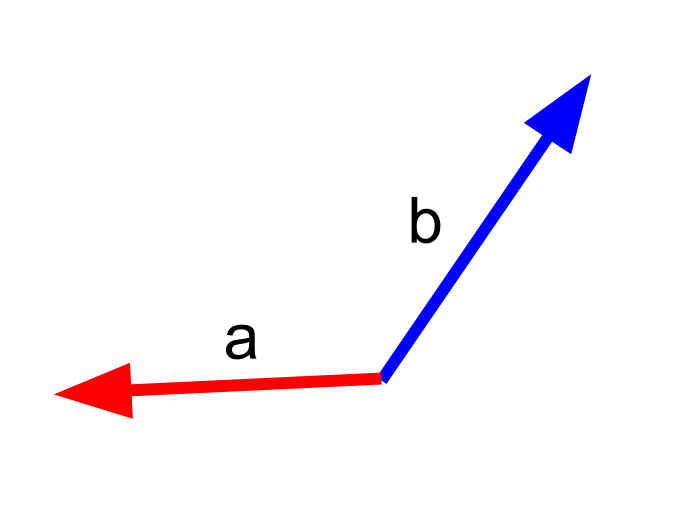
\includegraphics[scale=0.1]{Diagrams/vector5.png}\\
\hline

\end{tabular}
\caption{Table of turtle instruction symbols and their meaning to the interpreter}
\label{dot product test}
\end{table}
\FloatBarrier

\noindent
The cross product also known as the outer product takes two vectors and finds the perpendicular vector of the two vectors, this is only possible in 3D space and can be expressed in the following formula using the left-hand rule: 

\begin{equation}
a \times b = [(a_y b_z - a_z b_y), (a_z b_x - a_x b_z), (a_x b_y - a_y b_x)]
\end{equation}

\noindent
The result of a cross product can be seen in figure \ref{Cross product diagram} below. Where vectors $a$ and $b$ give the perpendicular vector $a \times b$. The cross product is very useful within physics calculations when it is necessary to find the rotational motion. 

\noindent
Some of the properties of the cross product are as follows:

\begin{itemize}
	\item is non-commutative, meaning order matters($a \times b \not= b \times a$).
	\item is anti-commutative ($a \times b = -(a \times b)$).
	\item is distributive with addition ($a \times (b + c) = (a \times b) + (a \times c)$).
\end{itemize}

\begin{figure}[htbp]
	{\centering
		\setlength{\fboxrule}{1pt}
		\vspace{7px}
		\fbox{
			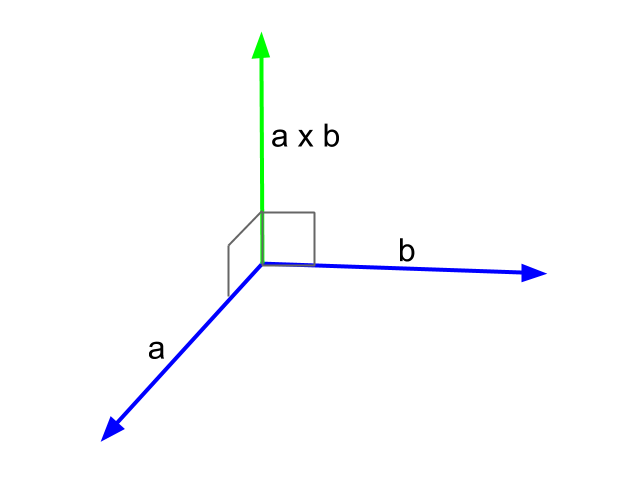
\includegraphics[scale=0.25]{Diagrams/cross_product.png}
			\label{Cross product diagram}
		}
		\caption{Diagram of the cross product of two vectors a and b.}
	}
\end{figure}
\FloatBarrier

\section{Matrices}

A model in 3D space will exist as a set of vertices which each have a position. Moving the model requires moving all of the the vertices of that model without distorting it in any way, this is called a model transform. There are four main types of transforms; translation, rotation, scale and shear. Matrices are a single matematical construct which is capable of carrying out all four of these transformations. This sections will only cover the first three as the shear transformation is likely not going to be useful for this thesis.    

A matrix is an 2D array of numbers, arranged into rows and columns, which can come in many different sizes. In 3D graphics, matrices used for transformations are the 3 $\times$ 3 and 4 $\times$ 4 matrix as seen below. A 3 $\times$ 3 matrix can be used for linear transorms such as scaling and rotation, furthermore, a linear transform which contains translation is known as an affine transform and can be represented by a 4 $\times$ 4 matrix known as an Atomic Transform Matrix. An atomic Transfom matrix is the concatination of four 4 $\times$ 4 matrices, one for translations, rotations, scale and shear transforms. Resulting in a 4 $\times$ 4 matrix as shown below. 

\begin{equation}
\textbf{M} = \begin{bmatrix}
M_{11} & M_{12} & M_{13} \\
M_{21} & M_{22} & M_{23} \\
M_{31} & M_{32} & M_{33}
\end{bmatrix}
\end{equation}

\begin{equation}
\textbf{M} = \begin{bmatrix}
M_{11} & M_{12} & M_{13} & M_{14}\\
M_{21} & M_{22} & M_{23} & M_{24}\\
M_{31} & M_{32} & M_{33} & M_{34}\\
M_{41} & M_{42} & M_{43} & M_{44}
\end{bmatrix}
\end{equation}

\noindent
The affine matrix can be shown in the expression below where $RS$ is a 3 $\times$ 3 matrix containing the rotation and scale where the $4^th$ elements are 0. The $T$ elements represent the translation with the 4th element being 1. 

\begin{equation}
\textbf{M} = \begin{bmatrix}
RS_{11} & RS_{12} & RS_{13} & 0\\
RS_{21} & RS_{22} & RS_{23} & 0\\
RS_{31} & RS_{32} & RS_{33} & 0\\
T_{1} & T_{2} & T_{3} & 1
\end{bmatrix}
\end{equation}

The product of two linear transform matrices will be another linear transform matrix that carries out both of those tranformations. This is true for the multiplication of two affine transform matrices as well, and is why matrix multiplication is so powerful in 3D graphics. Take the two matrices $A$ and $B$ which give the product $P$. In order to multiply $A$ and $B$ together, the dot product of the row and the column is calculated as seen below. It is also imporant to know that matrix multiplication is non-commutative $(AB \not= BA)$.

\begin{equation}
\textbf{AB} = \begin{bmatrix}
A_{11} & A_{12} & A_{13}\\
A_{21} & A_{22} & A_{23}\\
A_{31} & A_{32} & A_{33}
\end{bmatrix}
\times
\begin{bmatrix}
B_{11} & B_{12} & B_{13}\\
B_{21} & B_{22} & B_{23}\\
B_{31} & B_{32} & B_{33}
\end{bmatrix}
= \begin{bmatrix}
(A_{row1} \cdot B_{col1}) & (A_{row1} \cdot B_{col2}) & (A_{row1} \cdot B_{col3})\\
(A_{row2} \cdot B_{col1}) & (A_{row2} \cdot B_{col2}) & (A_{row2} \cdot B_{col3})\\
(A_{row3} \cdot B_{col1}) & (A_{row3} \cdot B_{col2}) & (A_{row3} \cdot B_{col3})
\end{bmatrix}
\end{equation}

To translate a vertex in 3D space without causing any distortion. The vertex can be added the the matrix below as follows. These translations can be carried out on all vertices in order to translate a whole object model. 

\begin{equation}
V + T = \begin{bmatrix}
V_{x} \\
V_{y} \\
V_{z}~ \\
1
\end{bmatrix}
+
\begin{bmatrix}
1 & 0 & 0 & 0\\
0 & 1 & 0 & 0\\
0 & 0 & 1 & 0\\
T_{x} & T_{y} & T_{z} & 1
\end{bmatrix}
= \begin{bmatrix}
(V_x + T_x)~ \\
(V_y + T_y)~ \\
(V_z + T_z)~ \\
1
\end{bmatrix}
\end{equation}

\noindent

In order to rotate a vertex in 3D space the vertex position and the rotation angle can be applied to the as a matrix depending on the axis about which it is rotating. These rotation matrices can be applied to the vertex itself in order to gain the new position of the vertex. 

\begin{equation}
R_x(\theta) = 
\begin{bmatrix}
(v_x)~ \\
(v_y)~ \\ 
(v_z)~ \\
1
\end{bmatrix}
\begin{bmatrix}
1 	& 0 					& 0 					& 0\\
0 	& \text{cos}(\theta) 	& \text{sin}(\theta) 	& 0\\
0 	& -\text{sin}(\theta) 	& \text{cos}(\theta) 	& 0\\
0 	& 0 					& 0 					& 1
\end{bmatrix}
\end{equation}

\begin{equation}
R_y(\theta) = 
\begin{bmatrix}
(v_x)~ \\
(v_y)~ \\
(v_z)~ \\
1
\end{bmatrix}
\begin{bmatrix}
\text{cos}(\theta) 	& 0 					& -\text{sin}(\theta) 	& 0\\
0 					& 1						& 0						& 0\\
\text{sin}(\theta) 	& 0 					& \text{cos}(\theta)	& 0\\
0 					& 0 					& 0 					& 1
\end{bmatrix}
\end{equation}

\begin{equation}
R_z(\theta) = 
\begin{bmatrix}
(v_x)~ \\
(v_y)~ \\
(v_z)~ \\
1
\end{bmatrix}
\begin{bmatrix}
\text{cos}(\theta) 	& \text{sin}(\theta) 	& 0						& 0\\
-\text{sin}(\theta) & \text{cos}(\theta) 	& 0
					& 0\\
0 					& 0 					& 1						& 0\\
0 					& 0 					& 0 					& 1
\end{bmatrix}
\end{equation}


\begin{equation}
ST = \begin{bmatrix}
S_{x} \\
S_{y} \\
S_{z} \\
1
\end{bmatrix}
\begin{bmatrix}
S_x & 0 & 0 & 0\\
0 & S_y & 0 & 0\\
0 & 0 & S_z & 0\\
0  & 0  & 0 & 1
\end{bmatrix}
= \begin{bmatrix}
(S_x R_x)~ \\
(S_y R_y)~ \\
(S_z R_z)~ \\
1
\end{bmatrix}
\end{equation}

\section{Quaternions}

In computer graphics there are a number of ways to represent 3D rotations. One method is to use matrix affine transforms, which is spoken about in the previous section. Matrices are a common way of represening rotation, however, it has a number of limitations. Matrices are represented by nine floating point values and can be computationally expensive to store and process, particularly when doing a vector to matrix multiplication. There are also situations where it is neccessary to smoothly interpolate from one rotation to another or to find the rotation somewhere between two different rotations. It is possible to make these calculations using matrices but it can become very complicated and even more computationally expensive. Quaterions are the answer to these challenges.

Quaternions look similar to a 4D vector. They contain four axes $q = [q_x, q_y, q_z, q_w]$, these are represented with a real axis ($q_w$) and three imaginary axes ($q_x, q_y, q_z$). A quaternion can be represented in the complex form below: 

\begin{equation}
q = (iq_x + jq_y + kq_z + qw)
\end{equation}

\noindent
For the purpose of this thesis it is not important to understand the derivation of quaterions in mathematics. However it is important to understand that any quaternion which obays the rule in \ref{unit quat} below is known as a unit quaternion.

\begin{equation} \label{unit quat}
	q_x^2 + q_y^2 + q_z^2 + q_w^2 = 1
\end{equation}

\noindent
Unit quaternions can be used for rotations, it is possible to convert a quaternion to a unit quaternion by taking the angle and the axis of a rotation and applying to the quaternion as seen in \ref{unit quat conversion}.

\begin{equation} \label{unit quat conversion}
\begin{aligned}
& q = [q_x, q_y, q_z, q_w]\\
& \text{where} \\
& q_x = a_x sin \frac{\theta}{2}\\
& q_y = a_y sin \frac{\theta}{2}\\
& q_z = a_z sin \frac{\theta}{2}\\
& q_w = cos \frac{\theta}{2}
\end{aligned}
\end{equation}

\noindent
The scalar part ($q_w$) is the cosine of the half angle, and the vector part ($q_x q_y q_z$) is the axis of that rotation, scaled by sine of the half angle of rotation. The unit quaternion can be used for rotations in a number of ways. The most useful of which is to rotate vectors, interpolate between two rotations and concatonate rotations together similar to how matrix transformations can be multiplied.

The first operation for quaternions is that of addition. The addition of two quaternions is quite simple, it involves taking each component of each quaternion and adding them together. This is similar to that of matrices addition and can be expressed as follows:

\begin{equation}
p + q = [(p_w + q_w), (p_x + q_x), (p_y + q_y), (p_z + q_z)]
\end{equation}

\noindent
Multiplication of quaternions is also incredibly powerful and can be used to concatonate rotations. There are a number of different types of quaternion multiplication, however, the one most commonly used for quaternion rotaton is called the grassmann product. This can be described in the following formula below. Where $p$ and $q$ are quaternions and the subscript $w$ indicates the scalar part and subscript $x, y, z$ indicate the vector components of each quaternion.

\begin{equation}
\begin{aligned}
& R = r_w + r_x + r_y + r_z\\
& \text{where}\\
& r_w = p_w q_w - (p_x q_x + p_y q_y + p_z q_z)\\
& r_x = p_w q_x + p_x q_w + p_y q_z - p_z q_y\\
& r_y = p_w q_y + p_y q_w - p_x q_z + p_z q_x\\
& r_z = p_w q_z + p_z q_w + p_x q_y - p_y q_x\\
\end{aligned}
\end{equation}

\noindent
To rotate a vector by a unit quaternion the vector will need to be converted into its quaternion form. This requires taking the unit vector $v$ and using it as the vector part of the quaternion with a scalar part being equal to zero. This can be written as $Q_v = [v, 0] = [v_x, v_y, v_z, 0]$. The grassmann product can be used to calculate the rotation, by taking the product of the rotation quaternion $q$ and the vector form quaternion $v$ and the inverse of the rotation quaternion $q^-1$. \\

\begin{equation}
	V_q = qvq^{-1}
\end{equation}

\noindent
For unit quaternions the conjugate and the inverse are identical. Quite simply the inverse of a unit quaternion can be calculated by negating the vector components of the quaternion whilst leaving the scalar component the same. This can be expressed as follows:

\begin{equation}
	q^{-1} = [-q_v, q_s]
\end{equation}

\noindent
Quaternion rotations can be concatonated together similar to how matrix transforms can be multiplied together in affine transforms. The grassman product is noncommutative and therefore order matters. Using the grassmann product the rotations can easily be multiplied together to give the result of all of those rotations as if they were to happen one after the other. This can be expressed as follows:

\begin{equation}
\begin{aligned}
Q_{net} = Q_3 Q_2 Q_1\\
v' = Q_3 Q_2 Q_1~ v~ Q_{1}^{-1} Q_{2}^{-1} Q_{3}^{-1}
\end{aligned}
\end{equation}

\noindent
The order by which the quaternions $Q_1, Q_2$ and $Q_3$ are applied is $Q_3$ then $Q_2$ and then $Q_1$. To apply this to a vector the product of the three quaternions is multiplied to the vector and then multiplied to the product of the inverse of each quaternion. 

Another incredibly useful mathematical function is called rotational linear interpolation also known as \acrshort{lerp}. The \acrshort{lerp} function takes two quaternions, $Q_1$ and $Q_2$ and linearly interperpolates between those two rotations by a given percentage  $\beta$. The \acrshort{lerp} function can be defined as follows.

\begin{equation}
\begin{aligned}
& Q_{\text{LERP}} = \text{LERP}(Q_1, Q_2, \beta) = \frac{(1-\beta)Q_1 + \beta Q_2}{\mid(1-\beta)Q_1 + \beta Q_2\mid} \\
& = \text{normalize} \left(\begin{bmatrix}
(1 - \beta) Q_{1x} + \beta Q_{2x}\\
(1 - \beta) Q_{1y} + \beta Q_{2y}\\
(1 - \beta) Q_{1z} + \beta Q_{2z}\\
(1 - \beta) Q_{1w} + \beta Q_{2w}					
\end{bmatrix}\right)
\end{aligned}
\end{equation}

\noindent
Using the linear interpolation function will result in a rotation between $Q_1$ and $Q_2$ at a given percentage $\beta$ that is between 0 and 1. Where 0 is the rotation of $Q_1$ and 1 is rotation of $Q_2$.

\section{summary}

This chapter covers the three major mathematical concepts used for representing 3D objects location, rotation and scale within a 3D graphics application. This includes moving objects around a scene for the purposes of animation or simulation. It is important to understand these concepts when implementing the string interpreter in order to be able to manipulate the branches or other objects. These concepts are also useful in the implementation of the physics simulations. The \acrlong{glm} (\acrshort{glm}) library provides a large number of useful classes and functions for working with vertices, matrices and quaternions.






